%======================================================================
%  Pape Saliou FALL – One-page CV
%======================================================================
\documentclass[11pt,a4paper]{article}

%---------- Encodage & langue ------------------------------------------
\usepackage[T1]{fontenc}
\usepackage[utf8]{inputenc}
\usepackage[british]{babel}

%---------- Géométrie --------------------------------------------------
\usepackage[left=2cm,right=2cm,top=2.2cm,bottom=2.2cm]{geometry}
\setlength{\parindent}{0pt}
\setlength{\parskip}{0pt}
\usepackage{setspace}
\setstretch{1.15}

%---------- Police & microtypographie ----------------------------------
\usepackage{FiraSans}
\renewcommand\familydefault{\sfdefault}
\usepackage[stretch=25,shrink=25,tracking=true]{microtype}

%---------- Icônes, couleur & images -----------------------------------
\usepackage{fontawesome5}
\usepackage{xcolor}
\usepackage{graphicx}
\definecolor{accent}{HTML}{161616}

%---------- Commandes pratiques ---------------------------------------
\newcommand{\headline}[1]{\textsc{\large #1}}
\newcommand{\sectiontitle}[1]{%
  \vspace{1em}\textbf{\uppercase{#1}}\par\vspace{.2em}
  \hrule height 0.7pt\relax\vspace{.8em}}

\newcommand{\job}[4]{% titre, entreprise, dates, bullets
  \textbf{#1} \hfill \faBuilding\;#2 \hfill \faCalendar\;#3\par
  \begin{itemize}\setlength\itemsep{.2em}#4\end{itemize}\vspace{.6em}}

\newcommand{\edu}[3]{% diplôme, établissement, dates
  \textbf{#1}\par
  {\small #2}\hfill\faCalendar\;#3\par\vspace{.8em}}

%======================================================================
\begin{document}\small

%------------------- En-tête : Nom, photo & tagline --------------------
\begin{center}
  \begin{minipage}[c]{0.73\linewidth}
    \Huge\bfseries Pape Saliou Fall\par
    \vspace{.2em}
    \textsc{Data Scientist junior}
  \end{minipage}%
  \begin{minipage}[c]{0.23\linewidth}
    \hfill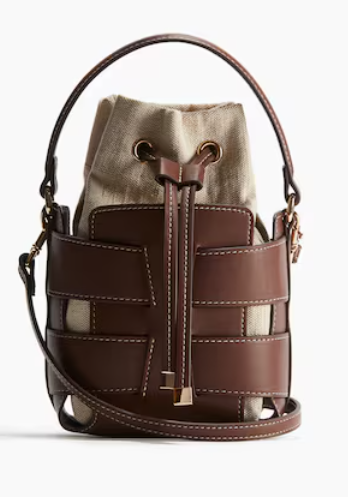
\includegraphics[width=\linewidth]{2883d8ffff7a4b87b28685096b56c64e.png}
  \end{minipage}
\end{center}\vspace{1em}

%------------------- Coordonnées --------------------------------------
\begin{tabular*}{\textwidth}{@{\extracolsep{\fill}}lll}
\faEnvelope[regular]\; papesalioufall2@gmail.com &
\faPhone\; 07 53 48 14 53 &
\faMapMarker*\; Paris, Île-de-France
\end{tabular*}

%------------------- Profil -------------------------------------------
\vspace{1.2em}
\fboxsep=8pt
\colorbox{gray!8}{%
  \parbox{\dimexpr\linewidth-2\fboxsep}{%
  \small Junior Data Scientist passionné par l’analyse de données et la construction de modèles prédictifs à forte valeur ajoutée. Solide maîtrise de Python, SQL et des bibliothèques de machine learning, complétée par une expérience pratique en visualisation de données et en déploiement de solutions. À l’aise dans la communication de résultats techniques à des parties prenantes non techniques et motivé par la résolution de problèmes complexes au sein d’équipes pluridisciplinaires.}}

%======================================================================
%                           EXPÉRIENCE
%======================================================================
\sectiontitle{Experience}

\job
  {Stagiaire Data Science}
  {Cursanova}
  {Jun.\,2022 – Mar.\,2023}
  {
    \item Développement de modèles de machine learning pour prédire la résiliation des abonnements.
    \item Collecte et nettoyage de jeux de données volumineux avec Python (Pandas, NumPy).
    \item Création de tableaux de bord interactifs sous Power BI pour la direction.
    \item Automatisation de pipelines ETL avec Airflow, réduisant le temps de traitement de 30 \%.
  }

%======================================================================
\begin{minipage}[t]{0.47\textwidth}
%=================== COMPÉTENCES ======================================
\sectiontitle{Skills}

\textbf{Programming \& Tools}\par
Python, R, SQL, Git, CI/CD, BigQuery,\linebreak
Pandas, NumPy, SciPy, scikit-learn,\linebreak
TensorFlow, PyTorch, Matplotlib, Seaborn,\linebreak
Power BI, Airflow,\linebreak
AWS, GCP.

\vspace{.6em}
\textbf{Data Science}\par
Machine Learning supervisé / non-supervisé,\linebreak
Deep Learning, Statistiques et probabilités,\linebreak
Data Visualization, ETL \& Data Pipelines.

\vspace{.6em}
\textbf{Languages}\par
Français (natif), Anglais (courant), Wolof (natif)

\vspace{.6em}
\textbf{Hobbies}\par
Football, échecs, électronique, lecture de science-fiction
\end{minipage}
\hfill
\begin{minipage}[t]{0.47\textwidth}
%=================== ÉDUCATION ========================================
\sectiontitle{Education}

\edu{Master 1 Data Science}{Sorbonne Université}{2022–2023}
\edu{Licence Mathématiques-Informatique}{Université Cheikh Anta Diop}{2018–2021}

%=================== CERTIFICATIONS ===================================
\sectiontitle{Certifications}

\edu{Google Data Analytics Professional Certificate}{Coursera}{Aug.\,2023}
\edu{AWS Certified Cloud Practitioner}{Amazon Web Services}{May 2024}

\end{minipage}

\end{document}